\documentclass[11pt]{article}
\usepackage[T1]{fontenc}
\usepackage[utf8]{inputenc}
\usepackage[margin=1in]{geometry}
\usepackage{amsmath,amssymb,booktabs,graphicx,hyperref,array}
\setlength{\emergencystretch}{2em}
\hypersetup{colorlinks=true,linkcolor=blue,citecolor=blue,urlcolor=blue}
\title{An Intervention-Response Subspace Retains Nearly All\\Readout-Relevant Prediction Error: A Case Study in Qwen3-0.6B}
\author{Rafa\l{} Wrona\\ \small Independent researcher}
\date{November 2026}
\begin{document}
\maketitle
\begin{abstract}
A rank-eight space fitted from native responses to an internal intervention, without readout labels, retains almost all of the readout-relevant part of a vector predictor's error. On fresh Qwen3-0.6B layer-21 contexts the historical predictor lies in this space, so oracle repair inside it inserts the projection of the true response: is/are readout MSE falls by 99.25\%, and its readout MSE is 0.47\% of that of inserting no response (relative RMS error about 6.9\%), although the space holds only 28\% of the vector-error energy. Post hoc, the space contains 29\% of the native readout-gradient energy, 37 times its random share, and the error outside it is nearly invisible to the locally linear readout; rank-eight principal subspaces of natural activations contain about 4\% and repair 7--8\%. The intervention was selected earlier for its is/are effect. Response spaces of three unscreened layer-19 neurons, even at matched response strength, repair only 0.2--3.6\%, like random spaces, so for the three tested alternatives the alignment does not transfer. Learning the correction helps, but restricting it to the space does not: prior-centered ridge reduces the historical predictor's MSE by 97.21\% with 384 labels, yet unrestricted ridge is better at 384 labels and, centered on the same prior, at 32 labels on a fourth fresh cohort, conditional on six fits of which one drives much of the difference. Other layers, frames and checkpoints show both benefit and harm of oracle repair.
\end{abstract}

\section{Introduction}
A model of an internal intervention is useful when its predicted vector change produces the right downstream effect. This study asks whether a response space selected from native vector data identifies a correctable component of prediction error, and whether that component can be learned well enough to help on new contexts. We follow the same prediction through vector error, oracle repair, learned correction, direct baselines and transfer.

The starting point is historical E041: on Qwen3-0.6B-Base, correcting error inside a rank-eight response space reduced the is/are readout MSE by 98.85\%, compared with 14.44\% outside. The original forecast favored outside repair and failed. The layer-21 regime is studied further because of this unexpected favorable outcome, so fresh cohorts test replication of a selected observation, not a randomly chosen layer. The intervened layer-19 coordinate was itself identified in earlier screening by its effect on the is/are readout. Four subsequent 64-block TEST cohorts separate replication of the oracle observation, learned correction, label-budget comparisons and a prior-matched comparison. A later three-fit/readout study probes the stability of the small-budget result on a reused cohort, and posthoc controls on the first cohort ask why the space works (Table~\ref{tab:scope}).

The central finding is that almost all of the readout-relevant prediction error lies in a low-rank space fitted to native intervention responses, while the larger error outside it is nearly invisible to the readout. Post hoc, this space captures 29\% of the readout-gradient energy against a random share of 0.8\%, while principal subspaces of natural activations capture about 4\% and repair only 7--8\% of the readout error. Moving from oracle diagnosis to learned prediction changes the conclusion. A space chosen without direct readout labels supports almost complete oracle correction on fresh lexical pairs. A learned prior-centered correction substantially improves the historical predictor on another fresh cohort. Full-vector direct ridge has lower mean loss at the matched additional training budget. A correction advantage at 32 labels appears in one fixed training sequence; three later FIT32 draws give mixed rankings, and on a fourth fresh cohort six new fits show no average advantage of C over Direct and a disadvantage against full-vector ridge centered on the same prior. Separate layer/frame tests include both benefit and harm. Together these results establish a useful empirical structure whose predictive and comparative value depends on the fitting and evaluation regime.

\begin{table}[ht]\centering\scriptsize
\setlength{\tabcolsep}{4pt}
\begin{tabular}{>{\raggedright\arraybackslash}p{.19\textwidth}>{\raggedright\arraybackslash}p{.36\textwidth}>{\raggedright\arraybackslash}p{.36\textwidth}}\toprule
Study & Data and reuse & Inference and role\\\midrule
L21 oracle/rank & First 64-block TEST; historical B5/$U$; rank controls use three disjoint eight-block FIT groups & Frozen operators and forecasts; nominal paired block intervals conditional on fixed fits.\\[3pt]
L21 learned384 & Second 64-block TEST; reuses all 24 FIT blocks, 384 vector labels & Prospective readout test; primary C-minus-P and secondary C-minus-Direct contrasts.\\[3pt]
L21 budget & Third 64-block TEST; one fixed FIT0/seed17 sequence at 32--256 labels, full pool at 384 & Prospective fixed-fit TEST; primary C32-minus-Direct32 contrast.\\[3pt]
Three FIT32/readout & Six new FIT blocks, three disjoint two-block fits; reuses budget TEST posthoc; adds have/has & Conditional nominal intervals; mixed per-fit rankings; readout transfer on the same contexts.\\[3pt]
Space controls & First TEST, cached native states; readout gradients through L22--27 & Posthoc, not yet independently reviewed; alternative label-free rank-8 spaces and one random draw scored through the native suffix.\\[3pt]
Prior-matched & Fourth 64-block TEST; six new disjoint 32-label FIT cohorts & Primary C32-minus-Direct\_P32, nominal interval conditional on six fits.\\[3pt]
Aligned and earlier tests & Qwen L27/Gemma-270M L17 share 256 lexical blocks; earlier Gemma-1B/Llama cohorts are separate & Three fixed fits/aligned model; nominal T5 intervals. Earlier single-fit families retain their original corrections.\\[3pt]
Forecast/diagnosis & Aligned Qwen; supporting 32-block scopes; historical/current Gemma fitted-object crosses & Descriptive sign/utility summaries and posthoc matrix substitutions.\\\bottomrule
\end{tabular}
\caption{Scope of the evidence. The four L21 TEST cohorts are distinct; the three-FIT32 study reuses the third. Conditions, fits and shared cohorts retain their dependence. The supplement gives complete protocols, chronology and result tables for the earlier studies; Appendix~A documents the posthoc space controls and the prior-matched study.}\label{tab:scope}
\end{table}

\section{Relation to existing work}
Engels et al.~\cite{engels2024} decompose and partially repair sparse-autoencoder reconstruction error, measuring downstream cross-entropy. Here the target is a native intervention delta and the outcome is squared error in its predicted grammatical logit-margin effect. The empirical extension is the linked sequence of response-space fitting, fresh oracle replication, rank/norm controls, learned correction and resource-aware baseline comparison.

Sharma et al.~\cite{sharma2026} analyze low-rank subspaces of behavioral interventions and their relation to decision directions; we instead ask which subspace of an intervention's native response carries the readout-relevant error of a vector predictor. Subspace activation patching, self-repair and computational-graph methods provide established context~\cite{makelov2023,rushing2024,ameisen2025,farnik2025}. End-to-end dictionary learning on downstream loss~\cite{braun2024} and gradient-based attribution patching~\cite{syed2023,kramar2024} likewise separate reconstruction or vector error from downstream-relevant change. The intervention edits a subject-number coordinate; number units and causal agreement mechanisms were studied earlier~\cite{lakretz2019,finlayson2021}. Deshpande~\cite{deshpande2026} studies preservation of refitted ridge readouts under sparse compression; our spaces instead derive from native vector responses and are tested by finite interventions through the native suffix. Guo et al.~\cite{guo2026} establish gradient-based intervention attribution and feature selection, directly preceding the gradient forecasting used here. Luo et al.~\cite{luo2026} show why intervention comparisons need strength, surface and basis matching. Our random-space and norm controls address specified parts of that comparison. Prior-centered ridge and kernel mean functions are standard regression constructions~\cite{rasmussen2006}; correcting a historical predictor in this way is hypothesis transfer learning with biased regularization~\cite{kuzborskij2013}, whose benefit with few target samples depends on how well the source hypothesis fits the target task; negative transfer is possible. Tanyel and Ayvaz~\cite{arxiv261105033} show that subspaces learned for a behavioral objective, such as distributed alignment search trained with cross-entropy, can exceed the effect of whole-state patching mainly because of the objective, and that to first order the effects of orthogonal parts add up to the whole. Our $U$ was fitted from vector responses without readout labels before that work appeared, and our in-space/out-of-space split of the linearized readout error uses the same first-order additivity; the intervention itself, however, was selected for its readout effect. The contribution rests on the measurements and their controlled comparisons.

\section{Prediction, correction and experimental design}
\subsection{Native response and oracle diagnostic}
For intervention $I$, let $D=y_I-y_0$ be the native target-branch output change. A target-free input representation predicts $P$. An orthonormal $U\in\mathbb R^{d\times r}$ holds the leading right singular vectors of the uncentered matrix of native FIT responses $D$; the historical space has $r=8$, chosen among ranks 1, 2, 4 and 8 by SELECT vector error without readout labels. Let $g_I(v)$ be the actual native-suffix logit margin after inserting $y_0+v$, holding the intervention's upstream residual fixed. With the same reference margin for target and prediction, squared error is
\[
 L(v)=[g_I(D)-g_I(v)]^2.
\]
The oracle diagnostics insert
\[
 P_U=P+UU^\top(D-P),\qquad P_{out}=D-UU^\top(D-P).
\]
Both access true TEST $D$. Inside repair removes the vector-error projection onto $U$, and outside removes its complement. Their downstream effects are measured through the suffix. If $e=g_I(D)-g_I(P)$ and $a=g_I(P_U)-g_I(P)$, the loss change is $a^2-2ea$. Positive change denotes worse prediction of the intervention effect.

The L21 experiments use Qwen3-0.6B-Base and the literal E041 upstream intervention. At the final prompt position, layer-19 SwiGLU coordinate 1317 moves toward its donor value at dose .5 or 1. Branch B leaves layer 20 free; branch C restores recipient coordinate 1423. Each lexical block has four subject/attractor-number forms and 16 branch/dose conditions. Donors reverse subject number in the F1 prompt, ``The \{subject\} that the \{attractor\} can see''. The target is layer-21 output; the exact native L22--27 suffix supplies the is/are readout. Native arithmetic is FP32, fitting/projection FP64, with separately qualified suffix batching. B5 uses a native ridge predictor.

The frozen input is $x=[\Delta x_{20}/s_{20},\Delta x_{21}/s_{21}]/\sqrt2$, and historical $P=\operatorname{FP32}(xWU^\top)$. These features require native upstream prefixes while avoiding the layer-21 output being predicted. TEST forecasts are globally frozen before the new native targets. The three new rank-study predictors use eight FIT blocks each (128 labels), fixed ridge penalty $10^{-4}$, six nested SVD ranks and fixed Gaussian-QR random spaces. A separate random arm rescales its correction to the FIT-space correction norm.

\subsection{C is ridge around a historical prior}
The learned correction fits coefficients of $(D-P)U$ and predicts $C=P+f_C(x)U^\top$. Same-$U$ fits $DU$; Direct fits full $D$. The shared estimator centers inputs and targets, uses $K+n\lambda I$, and adds the training target mean. Linear and RBF kernels use the grid $\lambda\in\{1,10^{-2},10^{-4},10^{-6}\}$; the RBF scale is the median positive training squared distance. Vector-only block CV selects models.

In exact arithmetic with $P=xWU^\top$, centered design $A=X-\bar X$ and $Y=DU$, the linear C fit is
\[
 \Gamma_C=\arg\min_\Gamma\big\{\|Y_c-A\Gamma\|_F^2+n\lambda\|\Gamma-W\|_F^2\big\},
 \qquad \widehat Y_C(x)=\bar Y+(x-\bar X)\Gamma_C.
\]
This is ridge centered on $W$, with an unpenalized intercept; same-$U$ shrinks toward zero. The implementation's FP32 P introduces a rounding qualification. RBF C is residual kernel ridge around mean function $xW+\overline{Y-XW}$. The supplement gives the exact smoother identities and implementation audit, including the conditions under which projected Direct equals same-$U$.

C and Direct search eight linear/RBF candidates in the learned384 and original budget studies; same-$U$ searches the four linear candidates. In the later three-FIT32 study, every method searches all eight. At 384 labels, all methods choose linear/$10^{-6}$, the grid's lower boundary. The original 32-label models all choose linear/$10^{-4}$. Two-block CV at 32 labels trains on one block per fold.

Historical information is a real resource. C inherits $W,U$ and scales; same-$U$ inherits $U$ and scales. E036's prior-development pool had 512 target rows across 128 documents with fitting and selection roles. Its ledger records 640 network, 640 CLT, 512 JVP and 512 target operations, beyond the subsequent vector-label budget. The supplement retains the full cost and selection chronology.

\subsection{Sampling, inference and companion data}
The independent sampling unit is the lexical block. The L21 analyses average 16 conditions within each of 64 blocks; aligned studies average fits and conditions within each of 256 blocks. Reported nominal 95\% intervals use the saved 1,999-draw paired block bootstrap and condition on fixed fitted objects. Original Gemma/Llama families retain their distinct saved correction rules. Each prospective stage through the three-FIT32 study has its own independent scientific completion receipt. The prior-matched study has an independent completion review (approved with changes; its completion package remains open). The space controls are a posthoc analysis, not yet independently reviewed, that fits principal subspaces and re-evaluates the native suffix and its gradient on cached states. Otherwise the manuscript uses saved analyses without refitting or resampling.

The companion transcoder study shares Qwen L27 states and 4,096 unit-dose native/first-fit ridge margins. Its ridge uses 128 FIT\_MAP labels; Direct256 here uses a different pooled training budget. The L21 cohorts and Gemma agreement tests have separate native acquisitions. Full reuse mappings and model identities are in the supplement.

\section{L21 results: repairability, usefulness and comparison}
\subsection{A vector-fitted space concentrates oracle benefit}
On the first fresh 64-block TEST, inside repair reduces historical B5 MSE by 99.25\%, compared with 8.38\% outside (Table~\ref{tab:oracle}). The inside-minus-B5 contrast is $-.0144172$, nominal 95\% interval $[-.0160698,-.0129072]$. Reductions range from 99.07\% to 99.30\% across the four branch/dose marginal groups. Because the historical predictor lies in the span of $U$ ($P=xWU^\top$), inside repair here inserts $UU^\top D$, the projection of the true response onto $U$: its residual .00010961 does not depend on $P$, whereas the percentage reduction does. Relative to inserting no MLP-21 change (MSE .02323977), the ratio $1-\mathrm{MSE}/\mathrm{MSE}_{\text{zero}}$ is 37.5\% for B5 and 99.53\% for the projection (an MSE-based ratio, not a share of effect amplitude; the projection's relative RMS error is about 6.9\%); on the second TEST the projection leaves 48\% of the mean squared response norm outside $U$ (Table~\ref{tab:learned}). The historical rank-eight vector-fitted space therefore retains almost all of the readout-relevant part of fresh responses while discarding about half of their energy.

\begin{table}[ht]\centering\small
\begin{tabular}{lrr}\toprule Historical fit/repair & Readout MSE & Reduction from B5\\\midrule
B5 prediction & .01452685 & ---\\
Oracle inside, rank 8 & .00010961 & 99.245\%\\
Oracle outside & .01330943 & 8.381\%\\
Full oracle & $1.31\times10^{-11}$ & Numerical floor\\\midrule
Zero MLP-21 change (reference) & .02323977 & 60.0\% higher\\\bottomrule\end{tabular}
\caption{First L21 TEST: 64 fresh blocks, 1,024 conditions, frozen historical fit. Oracle arms use true TEST error. Inside and outside have unequal rank/norm budgets; the full-oracle residual is the FP32 patch/suffix floor. Because $P$ lies in the span of $U$, inside repair equals inserting $UU^\top D$. The reference row inserts the natural MLP-21 output under the intervened residual.}\label{tab:oracle}
\end{table}

The separate three-fit rank study supplies controlled alternatives on the same TEST. Baseline MSE is .00075285. At rank eight, FIT-space repair gives .00008939, an 88.13\% reduction, versus 1.18\% for fixed equal-rank random spaces and 5.30\% for norm-rescaled random corrections. Each new predictor also lies in its own rank-eight FIT space, so rank-eight FIT-space repair again inserts the projection of $D$; its absolute residual, .00008939, is close to the historical .00010961, and the lower percentage reflects the new predictors' smaller errors. The saved FIT-space paired contrast is $-.00066347$, interval $[-.00081751,-.00052898]$. Figure~\ref{fig:ranks} retains all six ranks: the reductions rise to 94.14\% and 96.90\% at ranks 16 and 32. These controls support response-derived structure while also showing scope for larger spaces.

\begin{figure}[ht]\centering
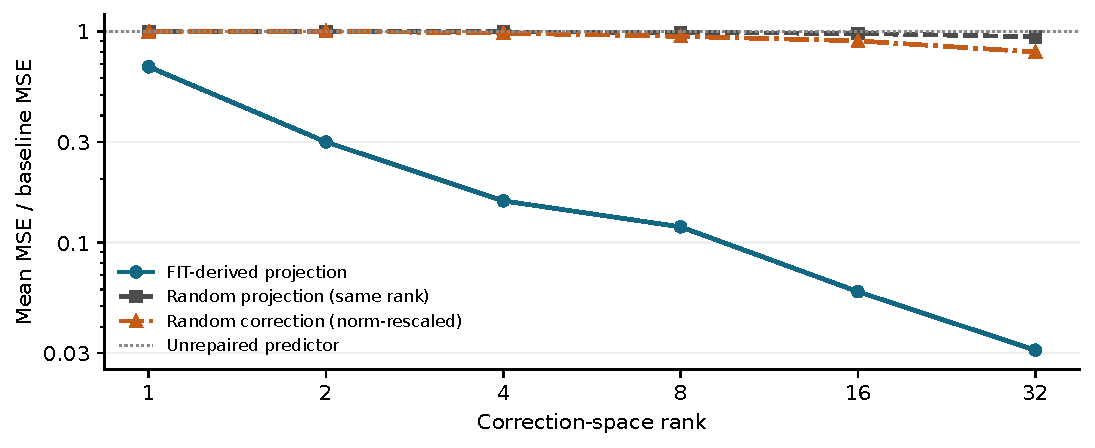
\includegraphics[width=.87\textwidth]{l21_rank_controls.pdf}
\caption{Three fixed new fits on the first 64-block TEST; means normalized by their common baseline. Rank and random seeds were fixed before outcomes. FIT-derived and random projections share rank; the rescaled arm matches correction magnitude. Points summarize these fixed controls.}\label{fig:ranks}
\end{figure}

\subsection{The out-of-space error is nearly invisible to the readout}
Two controls on the same first TEST ask why the historical space works. Both reuse the cached native states; the native readout gradient is computed by backpropagation through the exact L22--27 suffix at the predicted state $y_0+P$, and every repair is scored through that suffix. On average only 27.8\% of the vector-error energy $\|D-P\|^2$ lies in $U$ (mean of per-condition shares; MSE values are block-equal, the linearized shares below are pooled over conditions). Yet $U$ contains on average 29.1\% of the readout-gradient energy $\|g\|^2$ (per-condition range 11.7--44.8\%), against the random expectation $8/1024=0.78\%$. The readout error is almost exactly linear here: $g^\top(D-P)$ reproduces the finite error $g_I(D)-g_I(P)$ with pooled $R^2=.9997$. With $b_i=g_i^\top(D_i-P_i)$ and its in-$U$ term $a_i=g_i^\top UU^\top(D_i-P_i)$, the in-$U$ term carries the additive share $\sum_i a_ib_i/\sum_i b_i^2=95.5\%$ of the pooled second moment, and linearized inside repair removes $1-\sum_i(b_i-a_i)^2/\sum_i b_i^2=99.26\%$, matching the finite 99.25\%. The out-of-$U$ error, about 72\% of the vector-error energy, is therefore nearly invisible to the local readout. Rank-eight principal subspaces of the natural final-position MLP-21 outputs of the 96 FIT prompts of the rank study, or the subject-number class-mean difference plus seven principal directions, capture 3.6--4.1\% of the gradient and repair only 7.2--8.4\% of the readout error (Table~\ref{tab:spaces}). These posthoc measurements associate the 99\% repair with overlap between the response-fitted space and the readout-sensitive part of the error, not with the dominant variance of natural activations. They do not separate response variance from readout sensitivity: $U$ is itself the leading principal subspace of native responses, for an intervention selected earlier by its is/are effect. Moreover, unlike $U$, the alternative spaces do not contain $P$, so their inside repair is not a projection of $D$; inserting the projection $y_0+QQ^\top D$ without $P$ gives the same ordering (MSE .00011 for $U$ versus .021--.023 for every other-intervention space).

The decisive control asks whether any intervention's response space would do. Three layer-19 SwiGLU neurons drawn with a fixed seed (2356, 2177, 897), never screened on any readout, were moved toward their donor values on the same 96 FIT prompts and doses, and their native layer-21 responses were reduced by the same uncentered rank-8 SVD. Because these responses are weak (mean norm .013 versus about 2.6 for the historical intervention), a second variant moves each neuron by a calibrated shift that matches the historical response norm at each dose (mean norms 2.57--2.62). Both variants, jointly or per neuron, repair 0.2--3.6\% of the readout error and contain 0.3--1.6\% of the readout gradient, indistinguishable from 20 random spaces (mean repair 1.53\%, range $-0.36$ to 3.66\%). A space built from readout gradients themselves repairs 99.94\%, so the historical response space comes close to a label-informed ceiling without using readout labels. For the three alternative interventions tested, the alignment therefore does not appear; this does not establish specificity against all other interventions. Outside $U$, the mean absolute cosine between gradient and error components is .028, close to the value expected for unrelated isotropic directions (about $\sqrt{2/(\pi\cdot1016)}=.025$).

\begin{table}[ht]\centering\small
\begin{tabular}{lrr}\toprule Rank-8 space & Readout-MSE reduction & Gradient share\\\midrule
Historical $U$ (native responses) & 99.25\% & 29.1\%\\
PCA of natural outputs, uncentered & 8.43\% & 3.6\%\\
PCA of natural outputs, centered & 7.19\% & 3.7\%\\
Class difference + 7 PCA directions & 7.33\% & 4.1\%\\
Random (one draw; 20 draws: mean 1.53\%) & 2.94\% & 0.75\%\\
Other interventions, donor shift (3 neurons) & 0.93\% & 0.95\%\\
Other interventions, matched strength (3 neurons) & 2.74\% & 0.30\%\\
Gradient ceiling (top-8 PCA of FIT gradients) & 99.94\% & 96.3\%\\\bottomrule\end{tabular}
\caption{Oracle inside repair with alternative label-free spaces on the first L21 TEST (1,024 conditions, 64 blocks; equal-block MSE, base .014527). Gradient share is the mean fraction of native readout-gradient energy in the space; random expectation .78\%. The random row is one seeded draw and repairs B5's error; it is not comparable with the random arms of Figure~\ref{fig:ranks}, which repair the new predictors' much smaller errors. The $U$ row inserts $UU^\top D$ because $P$ lies in its span; other rows insert $P+QQ^\top(D-P)$. Posthoc, not yet independently reviewed: cached states with a fresh evaluation of the native suffix and its gradient.}\label{tab:spaces}
\end{table}

\subsection{Learned correction is useful against P; Direct384 has lower mean loss}
On a second fresh 64-block TEST, C trained on the existing 384 FIT vector labels reduces P's readout MSE by 97.21\% (Table~\ref{tab:learned}). Its primary C-minus-P contrast is $-.0149633$, nominal interval $[-.01669,-.01329]$. This is downstream improvement with forecasts frozen before true TEST error becomes available.

\begin{table}[ht]\centering\small
\begin{tabular}{lrr}\toprule Arm & Readout MSE & Vector squared error\\\midrule
Historical P & .01539272 & 4.08662\\
Prior-centered C & .00042944 & 2.89175\\
Same-$U$ direct & .00040599 & 2.88978\\
Direct384 & .00032652 & .29801\\
Mean correction & .01605005 & 4.07251\\
Oracle inside & .00008828 & 2.84390\\
Zero-change & .76689144 & 5.93717\\\bottomrule\end{tabular}
\caption{Second L21 TEST: 64 blocks and frozen fits using 384 reused vector labels. Vector error is mean squared L2. Oracle is diagnostic; zero-change predicts the original natural margin. Inference is conditional on fixed fits.}\label{tab:learned}
\end{table}

The secondary C-minus-Direct384 contrast is $+.000102919$, nominal interval $[+.000036397,+.000174289]$. Direct384 has 23.97\% lower mean loss than C; equivalently C has 31.52\% higher loss. Same-$U$ also has slightly lower point loss, while constant FIT-mean correction worsens P. C improves P across every reported branch/dose/subject/attractor marginal group. Direct384 has lower means in both branches and doses; one descriptive subject subgroup slightly favors C. Complete subgroup values remain in the supplement and evidence.

\subsection{A small-budget advantage depends on the fit}
A third fresh 64-block TEST compares one fixed FIT0/seed17 training sequence. Table~\ref{tab:budget} shows every budget. The 384-label models use the full pool, extending the lower-budget sequence with FIT0 blocks. At 32 labels, the primary C-minus-Direct contrast is $-.000809242$, nominal interval $[-.001215298,-.000446333]$: a 48.03\% MSE reduction. With the shared linear/$10^{-4}$ smoother, C versus same-$U$ differs through the historical prior; C versus Direct also changes the output span.

\begin{table}[ht]\centering\small
\begin{tabular}{rrrr}\toprule Vector labels & C & Same-$U$ & Direct\\\midrule
32 & .000875571 & .001435104 & .001684814\\
64 & .001275866 & .000927738 & .000790169\\
128 & .000767452 & .000696753 & .000481287\\
256 & .000489643 & .000496114 & .000440074\\
384 & .000342340 & .000321220 & .000308196\\\bottomrule\end{tabular}
\caption{Third L21 TEST: is/are MSE on 64 blocks, conditional on one fixed training sequence. $P=.015209579$. Direct has lower means at 64--384 labels; the 256/384 C-minus-Direct intervals include zero. The original learned384 study in Table~\ref{tab:learned} uses a different TEST cohort.}\label{tab:budget}
\end{table}

Three subsequent two-block FIT cohorts acquire 32 labels each and reuse this third TEST posthoc. On have/has, mean MSE is .001598713 for C and .001230636 for Direct: C-minus-Direct $+.000368077$, nominal interval $[+.000134272,+.000653699]$. On is/are, the mean contrast is $+.000172888$, interval $[-.000127204,+.000484746]$. Per-fit is/are contrasts are $+.000746091,-.000015488,-.000211940$; have/has contrasts are $+.000369036,+.001108920,-.000373724$. The mixed signs leave the original C32 advantage as an observation for one fixed training sequence, not a stable ranking across new fits and readouts.

A fourth fresh 64-block TEST then separates the prior from the correction procedure. Six new disjoint 32-label FIT cohorts train C, same-$U$, Direct and Direct\_P, a full-vector direct ridge centered on the same historical prior $P$; forecasts were frozen before the native targets. Mean is/are MSE is .001139 for Direct\_P, .001272 for same-$U$, .001340 for Direct and .001404 for C (P: .013777). The primary C-minus-Direct\_P contrast is $+.000265$, nominal block interval $[+.000148,+.000381]$ conditional on the six fits. It is less stable across fits: four of six favor Direct\_P, but one of these and one of the two C-favoring fits differ by less than $5\times10^{-5}$; without the most extreme fit the mean is $+.000074$, interval $[-.000026,+.000170]$; and a descriptive fit-level $t$ interval over the six fits, $[-.000252,+.000782]$, includes zero. With the prior equalized, restricting the correction to $U$ did not help on average on this cohort. Descriptive nominal secondary contrasts do not attribute the learned gain to the prior either. All four 32-label learners remove about 90\% of P's MSE. Adding the prior changes full-vector Direct by $-.000202$ ($[-.000412,+.000016]$) and the $U$-restricted fit by $+.000132$ (C minus same-$U$, $[-.000101,+.000382]$). The original primary C32-minus-Direct32 contrast, now repeated with six new fits on fresh contexts, is $+.000063$ ($[-.000229,+.000355]$; four of six fits favor C), so the earlier single-sequence advantage does not reappear on average. Learned correction is therefore useful against P, but at 32 labels neither the historical prior nor the restriction to $U$ gives it a demonstrated advantage over unrestricted ridge.

The supplementary implementation audit explains two numerical/semantic details of the three-FIT32 follow-up above, not of the fourth TEST below. Saved P vectors and is/are margins are identical to the budget study; its tiny P-MSE difference comes entirely from recomputing the native reference through another numerical path (maximum margin difference $1.90735\times10^{-5}$). The arm named zero inserts zero MLP21 delta while retaining the intervened residual, whereas earlier zero-change uses the original natural margin. All raw records are preserved.

\section{Transfer and policy results bound the interpretation}
The aligned layer-27 Qwen and layer-17 Gemma-270M tests use three fixed matched predictor/space pairs per model and the same 256 lexical blocks. The same three Qwen fitted pairs help on T2 and harm on T5 (Table~\ref{tab:aligned}); Gemma benefits on both frames. Outside-space repair has lower pooled loss in these cells, with a substantially larger dimension/norm budget. Per-fit reversals and full inside/outside tables are retained in the supplement.

\begin{table}[ht]\centering\small
\begin{tabular}{llrrl}\toprule Model & Frame & P MSE & Inside-minus-P & Nominal 95\% interval\\\midrule
Gemma-270M & T5 & .449097 & -.116462 & [-.144036,-.091732]\\
 & T2 & .209279 & -.126023 & [-.140182,-.113846]\\
Qwen-0.6B & T5 & .490827 & +.044905 & [+.013197,+.076805]\\
 & T2 & .672181 & -.139841 & [-.177426,-.107007]\\\bottomrule\end{tabular}
\caption{Aligned 256-block tests, conditional on three fits/model. T5 is primary; T2 is descriptive. Model, layer and fitting recipe differ from the L21 studies.}\label{tab:aligned}
\end{table}

Earlier separate single-fit 256-block tests establish T5 harm in Gemma-1B ($+.50370$, saved 99\% interval $[.43370,.57832]$, adjusted $p=.003$) and Llama-1B ($+.77826$, $[.66913,.89066]$, adjusted $p=.002$). Llama's secondary T2 effect is beneficial, $-.40679$ ($[-.47176,-.35053]$). Gemma's predicted vector/readout ranking reversal fails: the space removing more vector error also has lower fresh T5 readout loss. Posthoc old/new matrix substitutions show that the mean ranking follows the subspace-pair version on both fixed cohorts. The supplement preserves the full crossed table and original family definitions.

The separate L27 learned gate makes the distinction between sign forecasting and useful policy concrete. A local score $(Jc)^2-2(Jr)(Jc)$ uses native readout gradient $J$, residual $r=D-P$ and correction $c=UU^\top r$ to forecast finite loss-change signs. Replacing $r$ by a learned residual gives a deployable-with-prefix/gradient-access gate. On Qwen T5/T2, oracle sign accuracies are 99.479\%/99.837\%; learned accuracies are 64.746\%/68.620\%, versus constant-rule 63.249\%/59.375\%. Yet T5 gate loss .521107 exceeds P's .490827, and Direct256 has lower mean loss on both frames. These accuracies are dependent-cell descriptive fractions.

Supporting 32-block scopes reinforce that limit: learned sign accuracies on Gemma-1B/Llama-1B/Gemma-270M are 39.84\%/65.62\%/58.07\%, below constant-rule 60.94\%/72.40\%/62.50\%. Each learned gate loses to the better always/never policy. Complete loss tables, all matched crosses and timing qualifications are in the supplement.

\section{Limitations and interpretation}
The evidence concerns selected synthetic contexts, native branches and grammatical two-token margins. The intervened layer-19 coordinate was identified in earlier screening by its is/are effect, so a response space fitted without readout labels is still conditioned on a readout-selected intervention; response spaces of three unscreened interventions, including strength-matched versions, do not align with this readout. The MLP-21 response carries a small part of the intervention's readout effect (root-mean-square about .15 logit, versus about .9 logit for the whole intervention), and the space controls use one random draw and natural-activation principal spaces from 96 prompts. Fresh lexical pairs test the historically selected L21 regime; they leave model/frame/layer generalization conditional. The have/has extension changes a readout on reused prompts. Differences between L21, aligned and earlier tests also change operators and fitting recipes, so they cannot isolate layer as the cause of different repair signs.

Oracle correction requires true TEST error. Learned C avoids that access, while still requiring native upstream features and historical fitting information. Equal additional label budgets leave those prior resources unequal. The prior-matched Direct\_P comparison separates the prior from the output-span restriction, conditional on six fits; its fit-level interval includes zero and one fit drives much of the block-level difference. Kernel grids, fixed random draws and the three later FIT32 cohorts bound the conclusions to the tested choices.

Intervals condition on fitted objects and sample lexical blocks. The newer nominal analyses, older adjusted families and posthoc diagnostics have separate inferential scopes. In particular, two negative per-fit C32 contrasts coexist with a three-fit is/are interval crossing zero, and point rankings at budget256/384 leave the corresponding contrasts uncertain. Scientific completion approvals verify the recorded execution and evidence; external replication remains open.

The resulting thesis is specific. In the historically selected L21 regime, a rank-eight space fitted without readout labels to native responses of a readout-selected intervention retains almost all of the readout-relevant part of fresh responses while discarding about half of their vector energy, and it overlaps the native readout gradient far more than random or natural-activation principal spaces. This is a measured posthoc association, not an established mechanism, and three unscreened interventions of matched strength yield spaces with random-level repair. Other layers and models remain untested. At 32 labels, learned use of this structure gained no demonstrated advantage from the restriction to the space or from the historical prior over unrestricted ridge. Direct baselines, rank controls and transfer tests define where that usefulness holds. The supplementary report provides the complete historical record, forensic checks and operation receipts.

\paragraph{Use of AI tools.} AI assistants were used for code development, analysis support, literature search and editing of the text. All experimental designs, results and claims were checked by the author, who takes full responsibility for the content.

\paragraph{Code and data availability.} Code, frozen protocols, per-condition results, summary files and the full supplementary record are available at \url{https://github.com/rafalwronapl/interp-response-subspace}.

\clearpage
\small
\bibliographystyle{plain}
\bibliography{references}
\appendix
\section{Protocol summary}\label{app:protocol}
\textbf{Model and intervention.} Qwen3-0.6B-Base, FP32 native arithmetic, FP64 fitting and projection. At the final position of ``The \{subject\} that the \{attractor\} can see'', layer-19 SwiGLU coordinate 1317 is moved toward its donor value (dose .5 or 1); branch B leaves layer 20 free, branch C restores layer-20 coordinate 1423. Donors reverse subject number. The target is the layer-21 MLP output change $D$; readout is the is/are logit margin after the exact native layers 22--27, final norm and head, with the intervened upstream residual held fixed.

\textbf{Predictors and spaces.} Historical B5: ridge from target-free layer-20/21 input changes to the rank-8 response space $U$ obtained by SVD of native FIT responses (E036). Learned arms: C (coefficients of $(D-P)U$), same-$U$ ($DU$), Direct ($D$), Direct\_P (full-vector ridge centered on $P$); shared centered kernel-ridge estimator, linear/RBF kernels, $\lambda\in\{1,10^{-2},10^{-4},10^{-6}\}$, vector-only block cross-validation.

\textbf{Cohorts.} Four disjoint 64-block L21 TEST cohorts (each 256 prompts, 1,024 conditions): oracle/rank controls; learned384; label budget (reused post hoc for three FIT32 cohorts and a have/has readout); prior-matched (six new 32-label FIT cohorts). Lexical blocks are the resampling unit; intervals are 1,999-draw paired block bootstraps conditional on fixed fits. All forecasts were frozen before native TEST targets.

\textbf{Space controls.} Post hoc on the first TEST. Cached native states supply $y_0$, $D$ and the suffix inputs; the readout gradient is computed by backpropagation through layers 22--27 at $y_0+P$. Alternative rank-8 spaces: (i) uncentered and centered PCA of the natural final-position layer-21 outputs of the 96 FIT prompts; (ii) the subject-number class-mean difference plus seven PCA directions; (iii) 21 random Gaussian-QR spaces (one shown separately, 20 summarized); (iv) a gradient ceiling, the top-8 PCA of native readout gradients at the 384 cached FIT native endpoints; (v) other-intervention response spaces. For (v), new native forwards move layer-19 SwiGLU neurons 2356, 2177 and 897 (seeded draw, excluding 1317) on the 96 FIT prompts at doses .5 and 1, branch B: first toward their donor values, then by a calibrated shift toward the donor value whose size was set by bisection on eight FIT prompts so that the mean layer-21 response norm matches that of the historical intervention at each dose (1.717 and 3.429; shifts 3.70/7.32, 3.72/7.43 and 5.67/11.33). Each space is the uncentered rank-8 SVD of the stacked responses, jointly and per neuron. Every repair, with and without $P$, is scored through the exact suffix. These controls were run without a separate pre-run review; code and outputs: \texttt{analysis/A\_U\_gradient\_pca\_20261104} (\texttt{run.py}, \texttt{ctrl2.py}, \texttt{ctrl3.py}).

\section{Prior-matched experiment: per-fit contrasts}\label{app:prior}
\begin{table}[ht]\centering\small
\begin{tabular}{lrrrrrr}\toprule Contrast & FIT0 & FIT1 & FIT2 & FIT3 & FIT4 & FIT5\\\midrule
C$-$Direct\_P ($\times10^{-4}$) & 2.30 & 12.20 & 0.41 & $-$1.58 & $-$0.02 & 2.59\\
C$-$Direct ($\times10^{-4}$) & $-$1.74 & 13.54 & $-$6.57 & $-$1.72 & $-$2.41 & 2.69\\
Direct\_P$-$Direct ($\times10^{-4}$) & $-$4.04 & 1.34 & $-$6.97 & $-$0.14 & $-$2.39 & 0.10\\\bottomrule\end{tabular}
\caption{Fourth L21 TEST, is/are readout MSE differences per FIT cohort (64 blocks each). Positive values favor the second arm.}\label{tab:priorfits}
\end{table}
\end{document}
